%%%%%%%%%%%%%%%%%%%%%%%%%%%%%%%%%%%%%%%%%%%%%%%%%%%%%%%%%%%%%%%%%%%%%%%%%%%%%%%%%%%%
%Do not alter this block of commands.  If you're proficient at LaTeX, you may include additional packages, create macros, etc. immediately below this block of commands, but make sure to NOT alter the header, margin, and comment settings here. 
\documentclass[12pt]{article}
 \usepackage[margin=1in]{geometry} 
\usepackage{amsmath,amsthm,amssymb,amsfonts, enumitem, fancyhdr, color, comment, graphicx, environ}
\pagestyle{fancy}
\setlength{\headheight}{65pt}
\newenvironment{problem}[2][Problem]{\begin{trivlist}
\item[\hskip \labelsep {\bfseries #1}\hskip \labelsep {\bfseries #2.}]}{\end{trivlist}}
\newenvironment{sol}
    {\emph{Solution:}
    }
    {
    \qed
    }
\specialcomment{com}{ \color{blue} \textbf{Comment:} }{\color{black}} %for instructor comments while grading
\NewEnviron{probscore}{\marginpar{ \color{blue} \tiny Problem Score: \BODY \color{black} }}
%%%%%%%%%%%%%%%%%%%%%%%%%%%%%%%%%%%%%%%%%%%%%%%%%%%%%%%%%%%%%%%%%%%%%%%%%%%%%%%%%

\usepackage{tabto}
\usepackage{tikz}
\usepackage{tkz-berge}
\usepackage{indentfirst}
\usepackage{siunitx}
\usepackage{graphicx}
\usepackage{subfigure}
\usepackage{float}

%%%%%%%%%%%%%%%%%%%%%%%%%%%%%%%%%%%%%%%%%%%%%
%Fill in the appropriate information below
\lhead{Chenhao WU \\ 117010285}  %replace with your name
\rhead{Networks: Techonology, Economics and Society\\ EIE3280 Summer 2019 \\ Assignment 5} %replace XYZ with the homework course number, semester (e.g. ``Spring 2019"), and assignment number.
%%%%%%%%%%%%%%%%%%%%%%%%%%%%%%%%%%%%%%%%%%%%%

\begin{document}

\begin{problem}{1}
	\textit{Embedding trees}\par
	Consider a network of one server and $N = 3$ peers, given that (1) $ u_s = 2 $, $ u_1 = 3 $, $ u_2 = 2 $ and $ u_3 = 1 $ (all in Mbps), (2) all nodes have unlimited download capacity, and (3) each peer in a multi-cast tree can upload to any number of peers.\par
	(a) Find the maximum multi-cast rate $ r_{max} $. Draw a multi-tree that achieves this maximum. \par
	(b) Find the rate $ r_i $ of the $ i $th multi-cast tree, for all $ i = 1,\dots,T $, where $ T $ is the number of multi-cast trees from part (a). \par
	(c) Now consider a network with one server and $ N = 3 $ peers, with $ u_s = 3 $, $ u_1 = 3 $, $ u_2 = 2 $, and $ u_3 = 1 $ (in Mbps). But now we impose the constraint that each peer in a multi-cast tree can only upload to at most one peer, so as to limit the overhead in maintaining the states of the peers. Draw the resulting multi-tree that achieves the maximum multi-cast rate, and compute the per-tree rates $ r_i $.
\end{problem}

\begin{sol}
	(a) First we construct a maximum multi-cast tree according to the theoretical design of P2P network
	\begin{figure}[H]
		\centering
		\subfigure{}{
			\label{Fig. Experimental Data of Ex.1}
			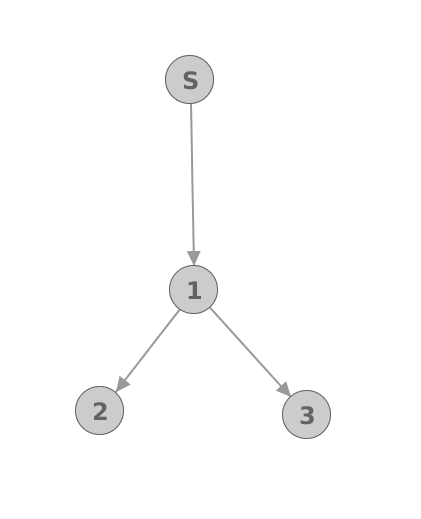
\includegraphics[width=0.3\textwidth, height=0.3\linewidth]{1.png}
			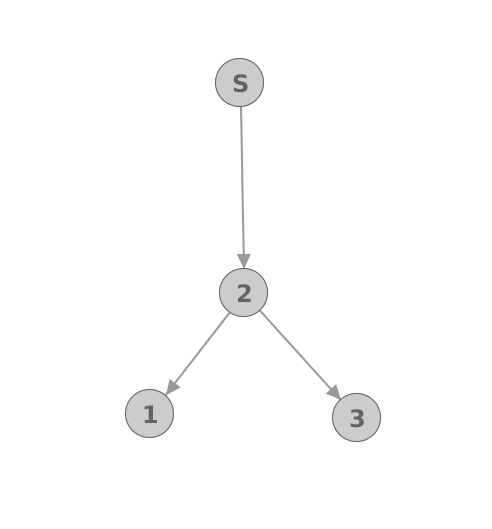
\includegraphics[width=0.3\textwidth, height=0.3\linewidth]{2.png}
			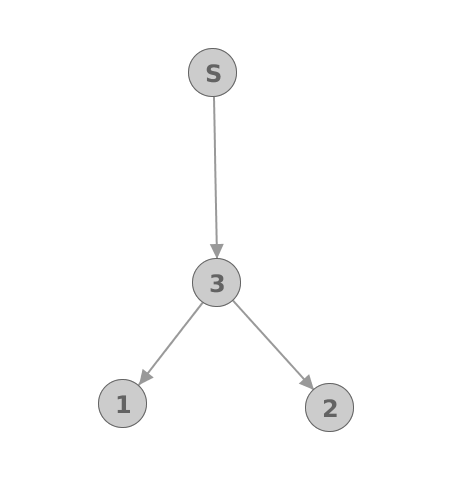
\includegraphics[width=0.3\textwidth, height=0.3\linewidth]{3.png}
		}
	\end{figure}
	according to mathematical analysis, without the consideration of user download speed, the maximum multi-cast rate $ r_{max} = \frac{1}{T} = \min\{u_s, \frac{u_s + \sum_i u_i}{N}\} = \min\{2, 8/3\} = 2$. \par
	(b) From previous calculation we conclude that $u_s \leq (u_s + \sum_{i=1}^Nu_i)/N$, thus in this case the rate of tree $i$ carry a rate $r_i = (\frac{u_i}{\sum_{j=1}^Nu_j})u_s$
	\begin{align*}
		u_1 &= \frac{3}{6} \times 2 = 1 \\
		u_2 &= \frac{2}{6} \times 2 = \frac{2}{3} \\
		u_3 &= \frac{1}{6} \times 2 = \frac{1}{3}
	\end{align*}
	(c). In this case the we are solving a single session problem that
	\begin{equation}
		\begin{aligned}
		\max \quad & r = \sum_{t\in T} y_t \\
		\textrm{s.t.} \quad & \sum_{t\in T}ty_t \leq C(v), \forall v \in V \\
		\end{aligned}
	\end{equation}
	where $y_t$ denotes the rate in subtree t, and $C_v$ denotes the maximum uplink capacity of node $v$. Notice that the problem is nonconvex, thus we need to reformulate the original problem into its dual problem
	\begin{equation}
		\begin{aligned}
		\min \quad & \sum_{v\in V} C_vp_v \\
		\textrm{s.t.} \quad & tp_v\geq 1, \forall t \in T 
		\end{aligned}
	\end{equation}
	where $p_v$ denotes the dual variable of node v. \par 
	A proposed algorithm to solve this problem from is as following \\
	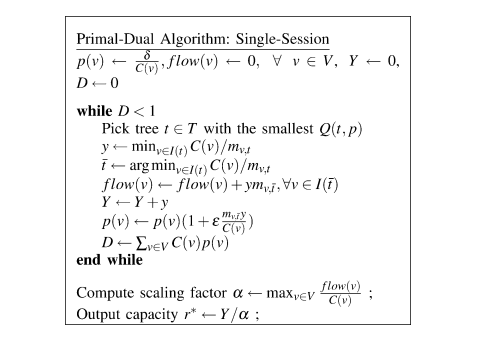
\includegraphics[width=0.5\textwidth]{5.png} \par
	By solving the dual problem according to the algorithm, we can obtain the maximum rate tree as following\\
	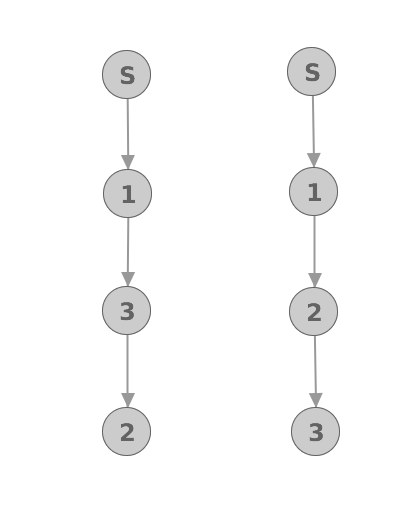
\includegraphics[width=0.4\textwidth]{7.png} \\
	where the rate of tree 1 is 1, and the rate of tree 2 is 2. 
\end{sol}

\begin{problem}{2}
	\textit{Aloha} \par
	There is a simpler random access protocol than CSMA that is just as famous. It is called \textbf{Aloha}, as it was invented in Hawaii in the early 1970s, and further led to the development of packet radio technologies. The operation of (the slotted time version of) Aloha is easy to describe. During each timeslot, each of a given set of $ N $ users chooses to transmit a packet with probability $ p $. We assume that if two or more users transmit at the same timeslot, all packets are lost. This is the only feedback available at each transmitter. Each lost packet is retransmitted with probability $ p $ too. We assume this process continues until a packet is eventually transmitted successfully. \par 
	(a) Assume the channel supports 1 unit of capacity (say, 1 Mbps) when there is a successful transmission. What is the throughput $ S $ as a function of $ N $ and $ p $? \par 
	(b) What is the optimal $ p $, as a function of $ N $, to maximize the throughput? \par
	(c) As the network becomes large and $ N\rightarrow\infty $, what is the maximized throughput? You will see it is not a big number, which is intuitive since slotted Aloha described above has neither the listen and wait nore the exponential backoff features. Aloha takes the least amount of communication and coordination and it does not even use carrier sensing. It also has a low throughput. CSMA leverages implicit message passing throughput can be high for a very small number of users but drops as the crowd gets larger. A centralized scheduler would have incurred even more coordination overhead, and would in turn provide the best performance. But in many networks, it is infeasible to afford a centralized scheduler.
\end{problem}
\begin{sol}
	(a) The probability of a successful transmission is calculated by 
	\begin{align*}
		S = Np(1-p)^{N-1}
	\end{align*}
	(b) Assume N is a constant and we obtain the first derivative of throughput $S$ that
	\begin{align*}
		\frac{dS}{dp} &= N((1-p)^{N-1} - (N-1)p(1-p)^{N-2})
	\end{align*}
	Setting the derivative equals to zero, we can obtain that 
	\begin{align*}
		p &= \frac{1}{N}
	\end{align*}
	and in this case 
	\begin{align*}
		S &= (1-\frac{1}{N}) ^ {N-1}
	\end{align*}
	(c) From previous calculation, we can obtain that the maximized throughput given $ N $ is $S = (1-\frac{1}{N}) ^{N-1}$. By calculating the value of maximized throughput limiting to infinity,
	\begin{align*}
		\lim_{N\rightarrow\infty} S &= \frac{1}{e}
	\end{align*}
	we can draw that when the network gets larger, the maximized throughput will converge to $\frac{1}{e}$
\end{sol}

\end{document}